\documentclass{beamer}
\usepackage{comment}
% wow this is a hack that lets you have more definitions in latex.
% see http://www.tex.ac.uk/cgi-bin/texfaq2html?label=noroom
\usepackage{natbib}
\usepackage{etex}
\usepackage{pgffor}
\usepackage[utf8]{inputenc}
%\usepackage[cyr]{aeguill}
\reserveinserts{28}
\usepackage{tikz}
\usepackage[customcolors]{hf-tikz}
%\usepackage[utf8]{inputenc}
%\mode<presentation>{\usetheme{Caltech}}

\usepackage{amsmath}
\usepackage{mathtools}
\usepackage{amssymb}
\usepackage{amsfonts}
\usepackage{amsthm}
\usepackage{multimedia}
\usepackage{color}
\usepackage{esint}
\usepackage{stmaryrd}
\usepackage{tabularx}
\usepackage{multirow}
\usepackage[squaren]{SIunits}
\usepackage{graphicx}
\usepackage{subfig}
\usepackage{diagbox}
\usepackage{pdfpages}
\usepackage{dsfont}
\usepackage{xcolor}
\usepackage{soul}
\usepackage[linesnumbered,ruled,vlined]{algorithm2e}


\newcommand{\mathcolorbox}[2]{\colorbox{#1}{$\displaystyle #2$}}



%%%%%%%%%%%%%%%%%%%%%%%%%%%%
% Paper dependent stuff    %
%%%%%%%%%%%%%%%%%%%%%%%%%%%%

\newcommand{\FTQ}{\textcolor{myalgocolor}{\normalfont \texttt{FTQ}}\xspace}
\newcommand{\FTQl}{\textcolor{myalgocolor}{\normalfont \texttt{FTQ}$(\lambda)$}\xspace}
\newcommand{\BFTQ}{\textcolor{myalgocolor}{\normalfont \texttt{BFTQ}}\xspace}
\newcommand{\ov}{\overline}
\newcommand{\oa}{\ov{a}}
\newcommand{\ox}{\ov{x}}
\newcommand{\oz}{\ov{z}}
\newcommand{\oy}{\ov{y}}
\newcommand{\os}{\ov{s}}
\newcommand{\ocS}{\ov{\cS}}
\newcommand{\ocA}{\ov{\cA}}

%%%%%%%%%%%%%%%%%%%%%%%%%%%%
% Aesthetics               %
% over-underline, hat, bold%
%%%%%%%%%%%%%%%%%%%%%%%%%%%%

\newcommand{\eps}{\varepsilon}
\newcommand{\vareps}{\varepsilon}
\renewcommand{\epsilon}{\varepsilon}
%\renewcommand{\hat}{\widehat}
\renewcommand{\tilde}{\widetilde}
\renewcommand{\bar}{\overline}

\newcommand*{\MyDef}{\mathrm{\tiny def}}
\newcommand*{\eqdefU}{\ensuremath{\mathop{\overset{\MyDef}{=}}}}% Unscaled version
\newcommand*{\eqdef}{\mathop{\overset{\MyDef}{\resizebox{\widthof{\eqdefU}}{\heightof{=}}{=}}}}


\def\:#1{\protect \ifmmode {\mathbf{#1}} \else {\textbf{#1}} \fi}
\newcommand{\CommaBin}{\mathbin{\raisebox{0.5ex}{,}}}

\newcommand{\wt}[1]{\widetilde{#1}}
\newcommand{\wh}[1]{\widehat{#1}}
\newcommand{\wo}[1]{\overline{#1}}
\newcommand{\wb}[1]{\overline{#1}}

% bf and bm missing due to conflict!!
\newcommand{\bsym}[1]{\mathbf{#1}}
\newcommand{\bzero}{\mathbf{0}}
\newcommand{\ba}{\mathbf{a}}
\newcommand{\bb}{\mathbf{b}}
\newcommand{\bc}{\mathbf{c}}
\newcommand{\bd}{\mathbf{d}}
\newcommand{\be}{\mathbf{e}}
\newcommand{\bbE}{\mathbb{E}}
\newcommand{\bg}{\mathbf{g}}
\newcommand{\bh}{\mathbf{h}}
\newcommand{\bi}{\mathbf{i}}
\newcommand{\bj}{\mathbf{j}}
\newcommand{\bk}{\mathbf{k}}
\newcommand{\bl}{\mathbf{l}}
\newcommand{\bn}{\mathbf{n}}
\newcommand{\bo}{\mathbf{o}}
\newcommand{\bp}{\mathbf{p}}
\newcommand{\bq}{\mathbf{q}}
\newcommand{\br}{\mathbf{r}}
\newcommand{\bs}{\mathbf{s}}
\newcommand{\bt}{\mathbf{t}}
\newcommand{\bu}{\mathbf{u}}
\newcommand{\bv}{\mathbf{v}}
\newcommand{\bw}{\mathbf{w}}
\newcommand{\bx}{\mathbf{x}}
\newcommand{\by}{\mathbf{y}}
\newcommand{\bz}{\mathbf{z}}

\newcommand{\bA}{\mathbf{A}}
\newcommand{\bB}{\mathbf{B}}
\newcommand{\bC}{\mathbf{C}}
\newcommand{\bD}{\mathbf{D}}
\newcommand{\bE}{\mathbf{E}}
\newcommand{\bF}{\mathbf{F}}
\newcommand{\bG}{\mathbf{G}}
\newcommand{\bH}{\mathbf{H}}
\newcommand{\bI}{\mathbf{I}}
\newcommand{\bJ}{\mathbf{J}}
\newcommand{\bK}{\mathbf{K}}
\newcommand{\bL}{\mathbf{L}}
\newcommand{\bM}{\mathbf{M}}
\newcommand{\bN}{\mathbf{N}}
\newcommand{\bO}{\mathbf{O}}
\newcommand{\bP}{\mathbf{P}}
\newcommand{\bQ}{\mathbf{Q}}
\newcommand{\bR}{\mathbf{R}}
\newcommand{\bS}{\mathbf{S}}
\newcommand{\bT}{\mathbf{T}}
\newcommand{\bU}{\mathbf{U}}
\newcommand{\bV}{\mathbf{V}}
\newcommand{\bW}{\mathbf{W}}
\newcommand{\bX}{\mathbf{X}}
\newcommand{\bY}{\mathbf{Y}}
\newcommand{\bZ}{\mathbf{Z}}

% calligraphic
\newcommand{\cf}{\mathcal{f}}
\newcommand{\cA}{\mathcal{A}}
\newcommand{\cB}{\mathcal{B}}
\newcommand{\cC}{\mathcal{C}}
\newcommand{\cD}{\mathcal{D}}
\newcommand{\cE}{\mathcal{E}}
\newcommand{\cF}{\mathcal{F}}
\newcommand{\cG}{\mathcal{G}}
\newcommand{\cH}{\mathcal{H}}
\newcommand{\cI}{\mathcal{I}}
\newcommand{\cJ}{\mathcal{J}}
\newcommand{\cK}{\mathcal{K}}
\newcommand{\cL}{\mathcal{L}}
\newcommand{\cM}{\mathcal{M}}
\newcommand{\cN}{\mathcal{N}}
\newcommand{\cO}{\mathcal{O}}
\newcommand{\cP}{\mathcal{P}}
\newcommand{\cQ}{\mathcal{Q}}
\newcommand{\cR}{\mathcal{R}}
\newcommand{\cS}{\mathcal{S}}
\newcommand{\cT}{\mathcal{T}}
\newcommand{\cU}{\mathcal{U}}
\newcommand{\cV}{\mathcal{V}}
\newcommand{\cW}{\mathcal{W}}
\newcommand{\cX}{\mathcal{X}}
\newcommand{\cY}{\mathcal{Y}}
\newcommand{\cZ}{\mathcal{Z}}

%%%%%%%%%%%%%%%%%%%%%%%%%%%%
% Math jargon              %
%%%%%%%%%%%%%%%%%%%%%%%%%%%%
\newcommand{\wrt}{w.r.t.\xspace}
\newcommand{\defeq}{\stackrel{\mathclap{\normalfont\mbox{\tiny def}}}{=}}
\newcommand{\maxund}[1]{\max\limits_{#1}}
\newcommand{\supund}[1]{\text{sup}\limits_{#1}}
\newcommand{\minund}[1]{\min\limits_{#1}}
\renewcommand{\epsilon}{\varepsilon}
\newcommand{\bigotime}{\mathcal{O}}


\DeclareMathOperator*{\argmin}{arg\,min}
\DeclareMathOperator*{\argmax}{arg\,max}
\DeclareMathOperator*{\cupdot}{\mathbin{\mathaccent\cdot\cup}}

%%%%%%%%%%%%%%%%%%%%%%%%%%%%
% Matrix operators         %
%%%%%%%%%%%%%%%%%%%%%%%%%%%%
\newcommand{\transpose}{^\mathsf{\scriptscriptstyle T}}
\newcommand{\transp}{\mathsf{\scriptscriptstyle T}}

%%%%%%%%%%%%%%%%%%%%%%%%%%%%
% Statistic operators      %
%%%%%%%%%%%%%%%%%%%%%%%%%%%%
\newcommand{\probability}[1]{\mathbb{P}\left(#1\right)}
\newcommand{\probdist}{Pr}
\DeclareMathOperator*{\expectedvalue}{\mathbb{E}}
\DeclareMathOperator*{\variance}{\text{Var}}
\newcommand{\expectedvalueover}[1]{\expectedvalue\limits_{#1}}
\newcommand{\condbar}{\;\middle|\;}
\newcommand{\gaussdistr}{\mathcal{N}}
\newcommand{\uniformdistr}{\mathcal{U}}
\newcommand{\bernoullidist}{\mathcal{B}}

%%%%%%%%%%%%%%%%%%%%%%%%%%%%
% Algebraic Sets           %
%%%%%%%%%%%%%%%%%%%%%%%%%%%%
\newcommand{\Real}{\mathbb{R}}
\newcommand{\Natural}{\mathbb{N}}
\newcommand{\statespace}{\mathcal{X}}
\newcommand{\funcspace}{\mathcal{F}}
\newcommand{\dynaspace}{\mathcal{T}}

%
%\newtheorem{theorem}{Theorem}
%\newtheorem{definition}{Definition}
%\newtheorem{lemma}{Lemma}
\newtheorem{proposition}{Proposition}
\newtheorem{remark}{Remark}
\newtheorem{conjecture}{Conjecture}
%\newtheorem{property}{Property}
%\newtheorem{assumption}{Assumption}
%\newtheorem{conjecture}{Conjecture}
%
%\newtheorem*{definition*}{Definition}
%\newtheorem*{theorem*}{Theorem}
%\newtheorem*{proposition*}{Proposition}
%\newtheorem*{remark*}{Remark}

\setbeamertemplate{footline}{%
\hfill%
\usebeamercolor[fg]{page number in head/foot}%
\usebeamerfont{page number in head/foot}%
\insertframenumber%
%\,/\,\inserttotalframenumber
\kern1em\vskip2pt%
}

\beamertemplatenavigationsymbolsempty

\author[shortname]{
Nicolas Carrara \inst{3} \and
Edouard Leurent\inst{3,5} \and
Tanguy Urvoy \inst{1} \and
Romain Laroche \inst{2} \and
Odalric-Ambrym Maillard \inst{3} \and
Olivier Pietquin \inst{3,4}}
\institute[shortinst]{\inst{1} Orange Labs\and %
\inst{2} Microsoft Montr\'eal. \and
\inst{3} Univ. Lille, CNRS, Centrale Lille, INRIA UMR 9189 - CRIStAL\and
\inst{4} Google Research, Brain Team, Paris\and
\inst{5} Renault}

\title[]{Budgeted Reinforcement Learning in Continuous State Space}
\date{10 august 2018.}
\begin{document}
    \begin{frame}
        \maketitle
        \centering
    \end{frame}

    \foreach \n in {0,1,2,3,4,5}{
    \begin{frame}{\textbf{Introduction} | Use-case}
        \begin{figure}
            \centering
            \includegraphics[scale=0.5]{img/\n}
        \end{figure}
    \end{frame}
    }

    \begin{frame}{\textbf{Introduction} | Use-case}
        \begin{block}{Problem}
            Given past trajectories, find a way to:
            \begin{itemize}
                \pause\item gather gold as much as possible;
                \pause\item limit the villager casualties under some budget;
                \pause\item being able to change the budget in real time.
            \end{itemize}

        \end{block}

        \pause
        \begin{block}{Solution}
            \begin{itemize}
                \item This problem can be cast as a Budgeted Markov Decision Process.
            \end{itemize}
        \end{block}
    \end{frame}


    \begin{frame}{Setting}
        \begin{block}{Markov Decision Process}
            We define a MDP as a tuple $(\cS, \cA, P, R_r, \gamma)$ where:
            \begin{itemize}
                \pause\item  $\cS$ is the state space, $\cA$ the action space,
                \pause\item $R_r\in\Real^{\cS \times \cA}$ the rewards,
                \pause\item $P\in \cM(\cS)^{\cS \times \cA}$ the dynamics, %  where $\cM(\mathcal{X})$ denotes the probability measures over a set $\mathcal{X}$
                \pause\item and $\gamma$ the discounted factor.
            \end{itemize}
        \end{block}
        \pause
        \begin{block}{Objective}
            \begin{itemize}
                \pause\item $G_r^\pi = \sum_{t=0}^\infty \gamma^t R_r(s_t, a_t)$ the $\gamma$-discounted return of rewards.
                \pause\item Find $\pi^*$ s.t $\forall s\in\cS$:
                \begin{equation}
                    \label{eq:mdp}
                    \begin{array}{lcr}
                        \displaystyle \pi^* \in \argmax_{\pi\in\cM(\cA)^\cS} \expectedvalue[G_r^\pi | s_0=s]
                    \end{array}
                \end{equation}

            \end{itemize}
        \end{block}
    \end{frame}

    \begin{frame}{Setting}
        \begin{block}{\textcolor{red}{Constrained} Markov Decision Process}
            We define a \textcolor{red}{CMDP} as a tuple $(\cS, \cA, P, R_r,\textcolor{red}{R_c}, \gamma,\textcolor{red}{\beta})$ where:
            \begin{itemize}
                \item  $\cS$ is the state space, $\cA$ the action space,
                \item $R_r\in\Real^{\cS \times \cA}$ the rewards, and $\textcolor{red}{R_c\in\Real^{\cS \times \cA}}$ the costs
                \item $P\in \cM(\cS)^{\cS \times \cA}$ the dynamics, %  where $\cM(\mathcal{X})$ denotes the probability measures over a set $\mathcal{X}$
                \item $\gamma$ the discounted factor, and $\textcolor{red}{\beta}$ the budget.
            \end{itemize}
        \end{block}

        \begin{block}{Objective}
            \begin{itemize}
                \item $G_r^\pi = \sum_{t=0}^\infty \gamma^t R_r(s_t, a_t)$ the $\gamma$-discounted return of rewards.
                \item \textcolor{red}{ $G_c^\pi = \sum_{t=0}^\infty \gamma^t R_c(s_t, a_t)$ the $\gamma$-discounted return of costs.}
                \item Find $\pi^*$ s.t $\forall s\in\cS$:
                \begin{equation}
                    \label{eq:cmdp}
                    \begin{array}{lcr}
                        \displaystyle \pi^* \in \argmax_{\pi\in\cM(\cA)^\cS} \expectedvalue[G_r^\pi | s_0=s] \\
                        \text{ s.t. }  \textcolor{red}{\expectedvalue[G_c^\pi | s_0=s] \leq \beta}
                    \end{array}
                \end{equation}
            \end{itemize}
        \end{block}
    \end{frame}

    \begin{frame}{Setting}
        \begin{block}{\textcolor{red}{Budgeted} Markov Decision Process}
            We define a \textcolor{red}{BMDP} as a tuple $(\cS, \cA, P, R_r,{R_c}, \gamma,\textcolor{red}{\cB})$ where:
            \begin{itemize}
                \item  $\cS$ is the state space, $\cA$ the action space,
                \item $R_r\in\Real^{\cS \times \cA}$ the rewards, and $R_c\in\Real^{\cS \times \cA}$ the costs
                \item $P\in \cM(\cS)^{\cS \times \cA}$ the dynamics, %  where $\cM(\mathcal{X})$ denotes the probability measures over a set $\mathcal{X}$
                \item $\gamma$ the discounted factor, and $\textcolor{red}{\cB}$ the budget space.
            \end{itemize}
        \end{block}

        \begin{block}{Objective}
            \begin{itemize}
                \item $G_r^\pi = \sum_{t=0}^\infty \gamma^t R_r(s_t, a_t)$ the $\gamma$-discounted return of rewards.
                \item  $G_c^\pi = \sum_{t=0}^\infty \gamma^t R_c(s_t, a_t)$ the $\gamma$-discounted return of costs.
                \item Find $\pi^*$ s.t $\forall (s,\textcolor{red}{\beta})\in\cS\times\textcolor{red}{\cB}$:
                \begin{equation}
                    \label{eq:bmdp}
                    \begin{array}{lcr}
                        \displaystyle \pi^* \in \argmax_{\pi\in\cM(\cA\times\textcolor{red}{\cB})^{\cS\times\textcolor{red}{\cB}}} \expectedvalue[G_r^\pi | s_0=s,\textcolor{red}{\beta_0=\beta}] \\
                        \text{ s.t. }  \expectedvalue[G_c^\pi | s_0=s,\textcolor{red}{\beta_0=\beta}] \leq \beta
                    \end{array}
                \end{equation}
            \end{itemize}
        \end{block}
    \end{frame}

    \foreach \n in {0,1,2,3,4}{
    \begin{frame}{The Dynamic Programming solution: intuition}
        \begin{figure}
            \centering
            %%\vspace{-1.5em}
            \includegraphics[scale=0.6,page=1]{img/a\n}
        \end{figure}
    \end{frame}
    }

    \begin{frame}{Augmented Settings}

        \textbf{Budgeted policies} $\pi$
        \begin{itemize}
            \pause\item Take a budget $\beta$ as an additional input
            \pause\item Output a next budget $\beta'$ 
            \pause\item $ \pi:\underbrace{(s,\beta)}_{\os} \rightarrow \underbrace{(a,\beta')}_{\oa}$
        \end{itemize}

        \textbf{Domain}
        \begin{itemize}
                \pause\item States $\ocS = \cS\times\cB$.
                \pause\item Actions $\ocA = \cA\times\cB$.
                \pause\item Dynamics $\ov{P}\left((s',\beta') \condbar (s,\beta), (a, \beta_a)\right) \eqdef P(s'|s, a)\delta(\beta' - \beta_a)$.
                \end{itemize}
        \textbf{2D  signals}
        \begin{enumerate}
            \pause\item Rewards $R = (R_r, R_c)$
            \pause\item Returns $G^\pi = (G_r^\pi, G_c^\pi)$
            \pause\item $V^\pi(\os) = (V_r^\pi, V_c^\pi) \eqdef \expectedvalue\left[ G^\pi \condbar \ov{s_0} = \os\right]$
                \pause\item $Q^\pi(\os, \oa)= (Q_r^\pi, Q_c^\pi) \eqdef \expectedvalue\left[ G^\pi \condbar \ov{s_0} = \os, \ov{a_0} = \oa\right]$
        \end{enumerate}
        
        \pause\textbf{Policy Evaluation}\\
        
        The Bellman Expectation equations% [\cite{Bellman}]
        are preserved, and the Bellman Expectation Operator $\cT^\pi$ is a $\gamma$-contraction.
    \end{frame}

    \begin{frame}{Augmented Optimality}
        \begin{definition}In that order, we want to:
\begin{enumerate}
    \item[(i)] \pause\colorbox{red}{Respect the budget $\beta$}: 
    \begin{equation*}
    \Pi_a(\os) \eqdef \{\pi\in\Pi: V_c^\pi(s, \beta) \mathcolorbox{red}{\leq \beta}\}
    \end{equation*}
    \item[(ii)] \pause\colorbox{green}{Maximise the rewards}:
    \begin{equation*}
        V_r^*(\os) \eqdef \mathcolorbox{green}{\max}_{\pi\in\Pi_a(\os)}  V_r^\pi(\os) \qquad\quad \Pi_r(\os) \eqdef \mathcolorbox{green}{\argmax}_{\pi\in\Pi_a(\os)}  V_r^\pi(\os)
    \end{equation*}
    \item[(iii)] \pause\colorbox{yellow}{Minimise the costs}: 
    \begin{equation*}
        V_c^*(\os) \eqdef \mathcolorbox{yellow}{\min}_{\pi\in\Pi_r(\os)}  V_c^\pi(\os), \qquad\quad \Pi^*(\os) \eqdef \mathcolorbox{yellow}{\argmin}_{\pi\in\Pi_r(\os)}  V_c^\pi(\os)
    \end{equation*}
\end{enumerate}

\pause We define the budgeted action-value function $Q^*$ similarly
\end{definition}
    \end{frame}

    \begin{frame}{Budgeted Bellman Optimality Equation}
        \begin{theorem}[Budgeted Bellman Optimality Equation]
            $Q^*$ verifies the following equation:
            \begin{align*}
                Q^{*}(\os, \oa) &= \cT Q^{*}(\os, \oa)\\
                &\eqdef R(\os, \oa) + \gamma \sum_{\os'\in\ocS} \ov{P}(\ov{s'} | \os, \oa)\sum_{\ov{a'}\in \ocA} \pi_\text{greedy}(\ov{a'}|\ov{s'}; Q^*) Q^{*}(\ov{s'}, \ov{a'}),
            \end{align*}
            where the greedy policy $\pi_\text{greedy}$ is defined by:
            \begin{align*}
                \pi_\text{greedy}(\oa|\os; Q) \in &\mathcolorbox{yellow}{\argmin}_{\rho\in\Pi_r^Q} \expectedvalueover{\oa\sim\rho}Q_c(\os, \oa), \\
                \text{where }\quad \Pi_r^Q \eqdef &\mathcolorbox{green}{\argmax}_{\rho\in\cM(\ocA)} \expectedvalueover{\oa\sim\rho} Q_r(\os, \oa) \\
                & \text{ s.t. }  \expectedvalueover{\oa\sim\rho} Q_c(\os, \oa) \mathcolorbox{red}{\leq \beta}
            \end{align*}
        \end{theorem}
    \end{frame}

    \begin{frame}{Optimality of the policy}
       \begin{proposition}[Optimality of the policy]
$\pi_\text{greedy}(\cdot~; Q^*)$ is \colorbox{yellow}{simultaneously optimal} in all states $\os\in\ocS$: $$\pi_\text{greedy}(\cdot~; Q^*)\in \mathcolorbox{yellow}{\Pi^*(\os)}$$

In particular, $V^{\pi_\text{greedy}(\cdot; Q^*)} = V^*$ and $Q^{\pi_\text{greedy}(\cdot; Q^*)}= Q^*$.
\end{proposition}

    \end{frame}

    \begin{frame}{Solving the untractable program}

        \begin{proposition}[$\pi_{\text{greedy}}=\pi_\text{hull}$]
            $\pi_\text{greedy}$ can be computed explicitly, as a mixture of two points that lie on the convex hull of $Q$.
        \end{proposition}
    \end{frame}

    \foreach \n in {0,1,2,3,4}{
    \begin{frame}{Solving the non-linear programming problem: intuition}
        \begin{figure}
            \centering
            %%\vspace{-1.5em}
            \includegraphics[scale=1.0,page=1]{img/b\n}
        \end{figure}
    \end{frame}
    }

    \begin{frame}{Not a contraction}
        \begin{theorem}[Non-Contractivity]
            For any BMDP ($\cS,\cA,P,R_r,R_c,\gamma$) with $|\cA| \geq 2$, $\cT$ is not a contraction.
            $$\forall\epsilon>0, \exists Q^1,Q^2\in(\Real^2)^{\ocS\ocA}:\|\cT Q^1-\cT Q^2\|_\infty \geq \frac{1}{\epsilon}\|Q^1-Q^2\|_\infty$$
        \end{theorem}
    \end{frame}

    \foreach \n in {0,1,2}{
    \begin{frame}{Not a contraction: intuition}
        \begin{figure}
            \centering
            %%\vspace{-1.5em}
            \includegraphics[scale=0.9,page=1]{img/d\n}
        \end{figure}
    \end{frame}
    }

    \begin{frame}{Contractivity on smooth $Q$-functions}
        \begin{conjecture}[Contractivity $\cL_\gamma$]
            $\cT$ is a contraction when restricted to the subset $\cL_\gamma$ of $Q$-functions such that "$Q_r$ is $L$-Lipschitz with respect to $Q_c$", with $L<\frac{1}{\gamma}-1$.
        \end{conjecture}

    \end{frame}

    \begin{frame}{Budgeted Dynamic Programming}
        \begin{algorithm}[H]
            \DontPrintSemicolon
            \KwData{$P, R_r, R_c$}
            \KwResult{$Q^*$}
            $Q_{0} \leftarrow 0$\;
            \Repeat{convergence}{
            $Q_{k+1} \leftarrow \cT Q_k$\;
            }
            \caption{Budgeted Value-Iteration}
        \end{algorithm}
    \end{frame}


    \begin{frame}{Budgeted Reinforcement Learning}

        We address several limitations of Budgeted Value-Iteration

        \begin{enumerate}
            \pause\item If the $P$, $R_r$ and $R_c$ are unknown:
            \begin{itemize}
                \pause\item Work with a {batch} of samples $\cD=\{(\os_i,\oa_i,r_i,\os_i'\}_{i\in [0,N]}$
                \pause\item Replace $\cT$ with a sampling operator $\hat{\cT}$:
                \begin{equation*}
                    \hat{\cT} Q(\os_i, \oa_i, r_i, \os'_i) \eqdef r_i + \gamma \sum_{\ov{a'_i}\in \cA_i} \pi_\text{greedy}(\ov{a'_i}|\ov{s'_i}; Q) Q(\ov{s'_i}, \ov{a'_i}).
                \end{equation*}
            \end{itemize}
            \pause\item If $\cS$ is continuous:
            \begin{itemize}
                \pause\item Employ function approximation $Q_\theta$, and minimise a regression loss
                $$\cL(Q_\theta, Q_\text{target};\cD) = \sum_{\cD} ||Q_\theta(\os, \oa) - Q_\text{target}(\os, \oa, r, \os')||_2^2$$
            \end{itemize}

        \end{enumerate}

    \end{frame}

    \begin{frame}{Budgeted Fitted-Q}
        \begin{algorithm}[H]
            \DontPrintSemicolon
            \KwData{$\cD$}
            \KwResult{$Q^*$}
            $Q_{\theta_0} \leftarrow 0$\;
            \Repeat{convergence}{
            $\theta_{k+1} \leftarrow \argmin_\theta \cL(Q_\theta, \hat{\cT} Q_{\theta_{k}}; \cD)$\;
            }
            \caption{Budgeted Fitted-Q Iteration}
        \end{algorithm}
    \end{frame}

    \begin{frame}{More scaling}

        \begin{itemize}
            \pause\item CPU parallel computing of the targets $\sum_{\ov{a'_i}\in \cA_i} \pi_\text{greedy}(\ov{a'_i}|\ov{s'_i}; Q) Q(\ov{s'_i}, \ov{a'_i})\ \forall i$
            \pause\item Same for samples generation.
            \pause\item Neural Network as function approximator: 
        \end{itemize}

        \begin{center}
            \resizebox{.7\textwidth}{!}{%
            
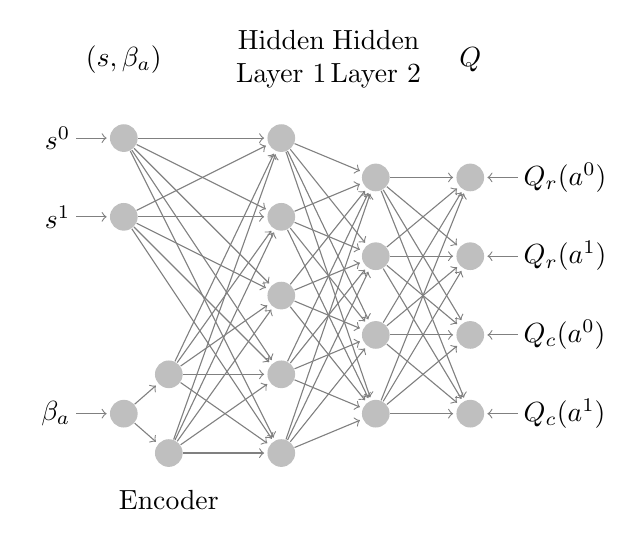
\begin{tikzpicture}[shorten >=1pt,->,draw=black!50, inner sep=1pt, node distance=\layersep]
        \tikzstyle{every pin edge}=[<-,shorten <=1pt]
        \tikzstyle{neuron}=[circle,fill=black!25,minimum size=10pt,inner sep=0pt]
        \tikzstyle{input neuron}=[neuron];
        \tikzstyle{input beta}=[neuron];
        \tikzstyle{qc}=[neuron];
        \tikzstyle{qr}=[neuron];
        \tikzstyle{hidden neuron}=[neuron];
        \tikzstyle{autoencoder neuron}=[neuron];
        \tikzstyle{annot} = [text width=4em, text centered]
        \tikzstyle{annot2} = [text width=10em, text centered]
        \def\layersep{2cm}
        % Draw the input layer nodes
        \foreach \name / \y in {0,...,1}
            \pgfmathtruncatemacro{\y}{0 + \y}
            \node[input neuron, pin=left:$s^\y$] (I-\name) at (0,-\y) {};

         % first layer
        \foreach \name / \y in {0,...,4}
        \pgfmathtruncatemacro{\y}{0 + \y}
            \path node[hidden neuron] (H1-\name) at (1*\layersep,-\y cm) {};

        \foreach \source in {0,...,1}
            \foreach \dest in {0,...,4}
                \path (I-\source) edge (H1-\dest);

        % BETA
        \node[input beta, pin=left:$\beta_a$] (BETA) at (0,-3.5) {};

        % beta auto encoder
        \foreach \name / \y in {0,...,1}
            \pgfmathtruncatemacro{\ybis}{3+ \y}
            \path node[autoencoder neuron] (AE-\name) at (\layersep/3.5,-\ybis cm) {};



        \foreach \name / \y in {0,...,3}
        \pgfmathtruncatemacro{\y}{0 + \y}
            \path[yshift=-0.5cm]
            node[hidden neuron] (H2-\name) at (1.6*\layersep,-\y cm) {};


        % actions
        \foreach \name / \y in {0,...,1}
        \pgfmathtruncatemacro{\y}{0 + \y}
            \path[yshift=-0.5cm] node[qr,pin=right:$Q_r(a^\y)$] (Qr-\name) at (2.2*\layersep,-\y cm) {};

        \foreach \name / \y in {0,...,1}
        \pgfmathtruncatemacro{\yy}{2 + \y}
            \path[yshift=-0.5cm] node[qc,pin=right:$Q_c(a^\y)$] (Qc-\name) at (2.2*\layersep,-\yy cm) {};

        \foreach \source in {0,...,1}
            \foreach \dest in {0,...,4}
                \path (AE-\source) edge (H1-\dest);



        \foreach \dest in {0,...,1}
            \path (BETA) edge (AE-\dest);

         \foreach \source in {0,...,4}
            \foreach \dest in {0,...,3}
                \path (H1-\source) edge (H2-\dest);

        \foreach \source in {0,...,3}
            \foreach \dest in {0,...,1}
                \path (H2-\source) edge (Qr-\dest);

         \foreach \source in {0,...,3}
            \foreach \dest in {0,...,1}
                \path (H2-\source) edge (Qc-\dest);
        % Annotate the layers
       \node[annot] (input) at (0,1) {$(s,\beta_a)$};
       \node[annot2] (input) at (\layersep/3.5,-4.6) {Encoder};
       \node[annot](h1) at (\layersep,1) {Hidden Layer 1};
       \node[annot](h2) at(1.6* \layersep,1) {Hidden Layer 2};
       \node[annot](output) at(2.2* \layersep,1) {$Q$};
        %\node[annot,right of=hl] {Output layer};
    \end{tikzpicture}

            }
        \end{center}

    \end{frame}




    \begin{frame}{Experiments: performances of BFTQ}
        \begin{itemize}
            \item Baseline: $\lambda$-FTQ, Lagrangian relaxation
            \begin{itemize}
                \item $R_r(s,a) \leftarrow R_r(s,a) - \lambda R_c(s,a) \text{ where } \lambda \geq 0$
            \end{itemize}.
            \item Applications:
            \begin{itemize}
                \item dialogue systems
                \item autonomous driving
            \end{itemize}
        \end{itemize}
    \end{frame}

    \begin{frame}{Experiments: dialogue systems}
        \begin{itemize}
            \item A slot-filling problem: the agent (the dialogue system) fills a form by asking the user each slot.
            \pause\item Two ways to deal with recognition errors:
            \begin{itemize}
                \item ask to repeat with voice (safe/slow);
                \item Ask to repeat with numeric pad. (unsafe/fast).
            \end{itemize}
        \end{itemize}

    \end{frame}
    \begin{frame}{Experiments: dialogue systems}
        \begin{center}
            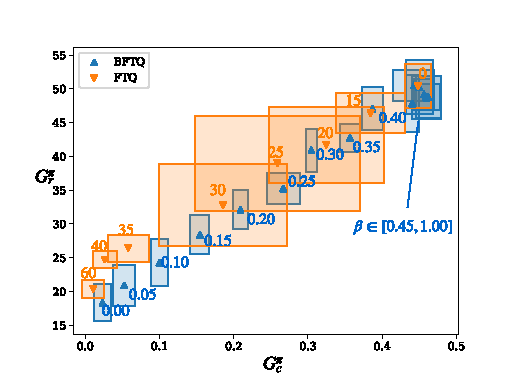
\includegraphics[width=\textwidth]{img/slot-filling.pdf}
        \end{center}
    \end{frame}


    \begin{frame}{Experiments: autonomous driving}
        \begin{itemize}
            \item the agent (the car) is on a two-way road with a car in front of it, two solutions: 
            \begin{itemize}
                \item it can stay behind (safe/slow);
                \item it can overtake (unsafe/fast).
            \end{itemize}
        \end{itemize}
    \end{frame}
    \begin{frame}{Experiments: autonomous driving}
        \begin{center}
            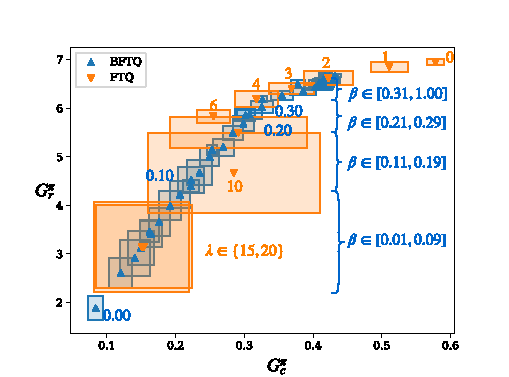
\includegraphics[width=\textwidth]{img/highway.pdf}
        \end{center}
    \end{frame}

    \begin{frame}{Experiments: autonomous driving}
        \href{scaling-up-brl.github.io-master/highway-env.html}{\beamergotobutton{BFTQ on the highway environment}}

    \end{frame}

    \begin{frame}{Risk-sensitive exploration}

        How to collect the batch $\cD$?

        \begin{itemize}
            \item We propose an $\epsilon$-greedy exploration procedure
            \begin{itemize}
                \pause\item Sample an initial budget $\beta_0$
                \pause\item At each step, where $\os=(s,\beta)$ only explore feasible budgets:
                \pause\begin{align*}
                    &\oa = (a, \beta_a)\sim\mathcal{U}(\Delta_{\cA\cB})\\
                    &\text{ where }  \Delta \text{ is such that }\probability{a, \beta_a|s, \beta} \text{verifies} \expectedvalue[\beta_a]\leq\beta
                \end{align*}
            \end{itemize}
        \end{itemize}


    \end{frame}

    \begin{frame}{Experiments: risk-sensitive exploration}

        \begin{itemize}
            \item Validate the risk-sensitive exploration procedure on the corridor environment
            \pause\item Learn 2 BFTQ policies with respectively:
            \begin{itemize}
                \item A batch generated by a risk-neutral $\epsilon$-greedy procedure
                \item A batch generated by a risk-sensitive $\epsilon$-greedy procedure
            \end{itemize}
        \end{itemize}
    \end{frame}


    \begin{frame}{Experiments: corridors}

        \begin{columns}
            \begin{column}{0.7\textwidth}
                \begin{itemize}
                    \item 2 corridors:
                    \begin{itemize}
                        \item high costs/high rewards around the starting state
                        \item no costs/low rewards around the starting state
                    \end{itemize}
                    \item The outermost cells are the ones yielding the most reward
                \end{itemize}
            \end{column}
            \begin{column}{0.3\textwidth}  %%<--- here
                \begin{center}
                    
\includegraphics[width=\textwidth]{img/env-corridor.pdf}
                \end{center}
            \end{column}
        \end{columns}

    \end{frame}


    \begin{frame}{Experiments: corridors}

        \begin{columns}
            \begin{column}{0.7\textwidth}
                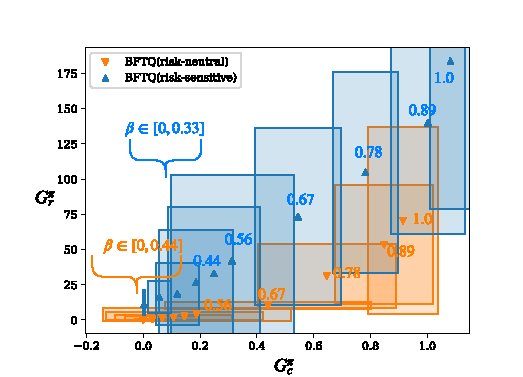
\includegraphics[page=1, width=\textwidth]{img/corridors}
            \end{column}
            \begin{column}{0.3\textwidth}  %%<--- here
                \begin{center}
                    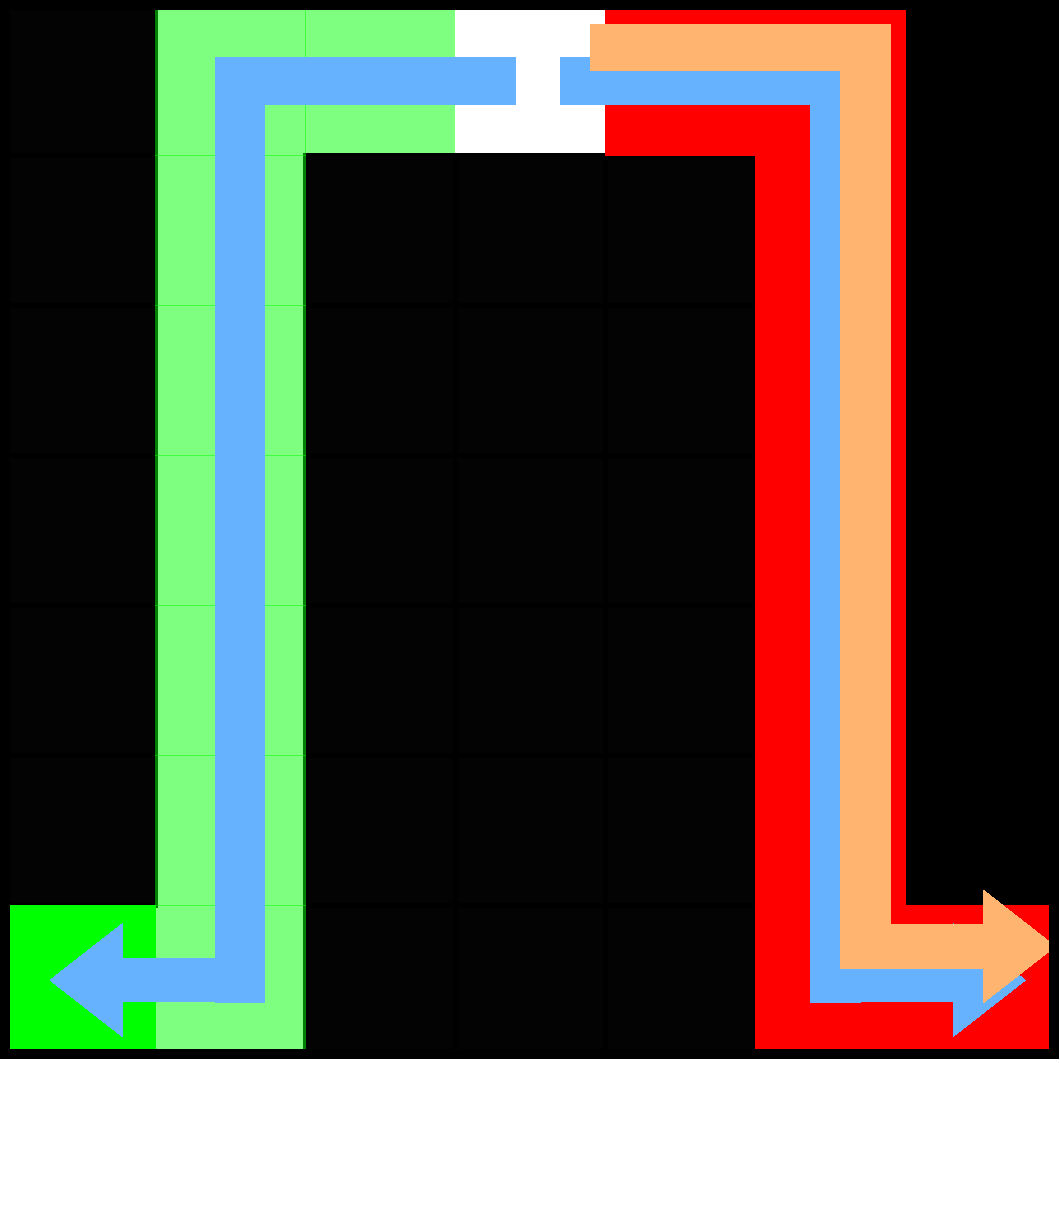
\includegraphics[width=\textwidth]{img/test.pdf}
                \end{center}
            \end{column}
        \end{columns}
    \end{frame}

    \begin{frame}{Experiments: corridors}
        \href{scaling-up-brl.github.io-master/corridors.html}{\beamergotobutton{Risk-sensitive vs Risk-Neutral on the corridors environment}}

    \end{frame}


    \begin{frame}{Summary}

        \begin{enumerate}[+]
            \pause\item<1-> Budgeted Bellman Optimality Operator.
            \begin{itemize}
                \pause\item Fixed point.
                \pause\item Not a contraction but converging in practice.
            \end{itemize}
            \pause\item<2-> Scalable for RL in continuous state space.
            \begin{itemize}
                \pause\item Function approximation with Neural Network (dedicated architecture).
                \pause\item Solving of the untractable program using convex hull.
                \pause\item CPU parallel computing of the target.
                \pause\item Risk-sensitive exploration procedure.
            \end{itemize}

            \pause\item<3-> Experiments on two applications.
            \begin{itemize}
                \pause\item BFTQ reaches similar performances as Lagrangian relaxation,
                \pause\item with no need for calibration,
                \pause\item and less variance.
            \end{itemize}
        \end{enumerate}

    \end{frame}

\end{document}

